\section{Algorithms}

\cprotect\subsection{1. Octree From Distributed Point Set - \verb|Points2Octree|}

\begin{frame}
\frametitle{Points2Octree}
\begin{itemize}
    \item \textbf{Goal}: Go from a set of points distributed across processors to an *unbalanced distributed octree.
    \item State of the art software tends to use linear trees - i.e. only store leaf nodes \cite{Malhotra2016,Isaac,Lashuk2009,Sundar2013,Sundar2007}
    \item We implement the scheme outlined in \cite{Sundar2007} augmented with extra features for use with FMM and other solvers using \textbf{Rust} and MPI.
\end{itemize}
\end{frame}

\begin{frame}
    \frametitle{Octrees}
    \begin{itemize}
        \item Represent each node uniquely with an anchor and its level in the tree.
        \item e.g. the anchor of d is (4, 2) and it's at level 3.
        \item Can represent uniquely with tuple (4, 2, 3).
    \end{itemize}

    \begin{figure}
        \centering
        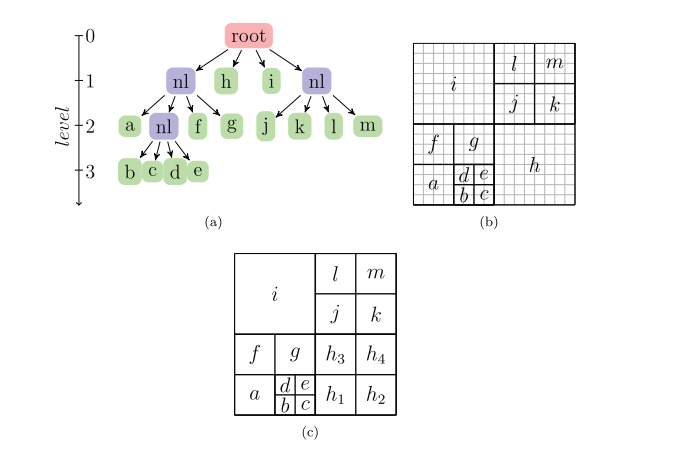
\includegraphics[width=8.5cm]{assets/anchor.png}
        \label{fig:anchor}
        \caption{Adapted from \cite{Sundar2007}}
    \end{figure}
\end{frame}

\begin{frame}
    \frametitle{Nice Properties of Morton Encoding}
    \begin{itemize}
        \item Sorting leaves in ascending order of Morton keys is equivalent to pre-order traversal of the leaves. Connecting centres, we observe a `Z' pattern.
        \item Encoding preserves spatial locality.
        \item Given octants $a$ $b$ and $c$ with $a < b < c$ and $c \notin \{ \mathcal{D}(b) \}$ $\implies a < d < c, \> \forall d \in \{ \mathcal{D}(b) \} $
    \end{itemize}
\end{frame}

\begin{frame}
    \frametitle{Briefly on Rust}
    \begin{itemize}
        \item Offers memory safety (compile time checks for memory violations).
        \item Does away with complex programming models (object orientation).
        \item (Relatively...) Simple API, can feel like writing in an interpreted language.
        \item Interfaces nicely with other languages, and their libraries. e.g. mature (open source) support for MPI.
        \item Simple cross platform build system (Cargo).
        \item `Zero Cost Abstractions' - performance won't suffer for using handy abstractions (map, filter, fold ...).
    \end{itemize}
\end{frame}

\begin{frame}
    \frametitle{Points2Octree - Algorithm}
    \small
    \begin{enumerate}
        \item Apply Morton encoding to points at each processor.
        \item Perform a parallel sort, and remove duplicate Keys, associate points and Keys. Dominates complexity of algorithm \cite{Sundar2007}.
        \item Find \textit{coarsest possible} tree that spans the domain defined by the Keys at each processor.
        \item Find the \textit{coarsest} node(s) at each processor. Complete the region in between the coarsest node(s) across each processor - known as the \textbf{blocks}.
        \item Perform some kind of load balancing over block, and redistribute the blocks.
        \item Split blocks to find final distributed octree.
    \end{enumerate}
\end{frame}


\begin{frame}
    \frametitle{Illustration of Blocks}
    \begin{figure}
        \centering
        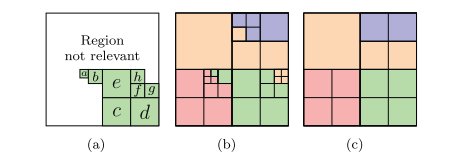
\includegraphics[width=8.5cm]{assets/blocks.png}
        \label{fig:anchor}
        \caption{Adapted from \cite{Sundar2007}}
    \end{figure}
\end{frame}

\cprotect\subsection{2. 2:1 Balance/Load Balancing Octree - \verb|BalanceOctree|}

\begin{frame}
    \frametitle{2:1 Balancing}
    \begin{figure}
        \centering
        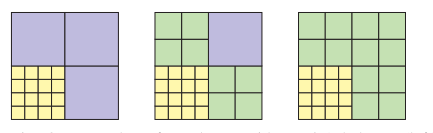
\includegraphics[width=8.5cm]{assets/balance.png}
        \label{fig:balancing}
        \caption{Adapted from \cite{Suh2020}}
    \end{figure}
\end{frame}

\begin{frame}
    \frametitle{2:1: Balancing}
    Not always strictly necessary (e.g. particle FMM). However, essential to offer functionality in any octree library. Tends to dominate runtime, run as post-processing step.
    \begin{enumerate}
        \item E.g. evaluating near interaction in volume (continuous medium) FMM $\int_{Near Field} K(x,y) f(y)$ is computationally expensive (many singular/near singular integrals), balancing allows one to use precomputed tables for valid interactions \cite{Malhotra2016}.
        \item Other numerical schemes may take advantage of it to maximise accuracy while minimising memory footprint \cite{Suh2020}.
    \end{enumerate}
\end{frame}

\begin{frame}
\frametitle{Options for Balancing}
    Two major algorithmic approaches to balancing
    \begin{enumerate}
        \item (older) \textit{Ripple} based algorithms \cite{Isaac,Sundar2007}.
        \item (newer) Sorting based algorithms \cite{Malhotra2016,Lashuk2009}.
    \end{enumerate}
\end{frame}

\begin{frame}
    \frametitle{2:1 Balancing - (1) Ripple Based}
    \begin{enumerate}
        \item Each process enforces balance in its subdomain, must communicate with neighbours to resolve conflicts.
        \item Generally require multiple rounds of communication.
        \item Algorithmically fairly complex, with no clear advantage of sorting based methods \cite{Suh2020}.
        \item Existing OS software: P4EST (C++)
        \item Won't talk about them further.
    \end{enumerate}
\end{frame}

\begin{frame}
    \frametitle{2:1 Balancing - (2) Sorting Based}
    \begin{enumerate}
        \item Each process computes a tree over global domain that's suitably balanced with the octants it controls.
        \item These are then sorted in parallel, and duplicates/overlaps are removed (favouring the smaller octants). Guaranteed to be 2:1 balanced.
        \item Simple communication pattern (sorting).
        \item Existing OS software: Dendro (C++)
    \end{enumerate}
\end{frame}

\begin{frame}
    \frametitle{2:1 Balancing - Sequential Algorithm}

    Example local balancing algorithm (there are numerous approaches):


    1. Balance Subroutine

    for $i \leftarrow L_{max} \> to \>  1$ do
    \begin{enumerate}
        \item For each octant at this level, find coarsest compatible neighbours, add to output.
    \end{enumerate}

    2. Remove overlaps

    for $i \leftarrow L_{max} \> to \>  1$ do
    \begin{enumerate}
        \item For each octant at this level, remove any ancestors that lie in the tree.
    \end{enumerate}

\end{frame}

\subsection{3. Parallel Sorting Algorithm}

\begin{frame}
    \frametitle{Choosing a Sorting Algorithm}
    This is the most important choice, as both building and balancing require a parallel sort, and in both cases will dominate runtime.
\end{frame}

\begin{frame}
    \frametitle{State of the Art - HykSort}
    First presented in 2013 \cite{Sundar2013}, remains fastest method in 2021 \cite{Suh2020}.

    \begin{enumerate}
        \item Sample Sort contains a global AllToAll communication. This leads to network congestion for larger problems.
        \item Requires selection (and parallel sorting) of $p-1$ splitters, where $p$ is the number of processors. Can be expensive for large $p$.
        \item HykSort uses a Hypercube style communication pattern, but with $k$ rather than 2 splits for each recursive call, where $k < p$, $k\beta$ splitters are chosen.
    \end{enumerate}
\end{frame}

\begin{frame}
    \begin{figure}
        \centering
        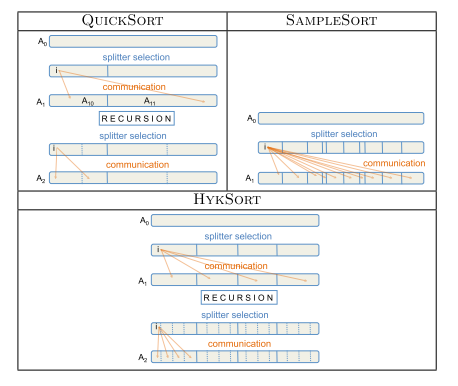
\includegraphics[width=8.5cm]{assets/hyksort.png}
        \label{fig:hyksort}
        \caption{Adapted from \cite{Sundar2013}}
    \end{figure}
\end{frame}

\begin{frame}
    \begin{enumerate}
        \item In \cite{Sundar2013} they sort 8 trillion 32 bit integers in 37 seconds on 262,144 cores.
        \item Use OpenMP optimised local sorting algorithm based on merge sort, and SIMD optimised merge operation. Don't report similar benchmark for sorting Morton keys though.
    \end{enumerate}
\end{frame}